
\subsection{Os desafios}

Este projeto apresentou-nos diversos desafios. Foi necessário investigar mais sobre:
\begin{itemize}
	\item A melhor abordagem de implementação do API;
	\item A base de dados mais adequada e formas de garantir estabilidade da configuração nos ambientes de desenvolvimento dos membros da equipa;
	\item Acessos concorrentes instâncias de objetos e persistência dos dados;
	\item Persistência dos dados (objetos em memória e na base de dados);
	\item Implementação de classes e código Thread-Safe;
	\item Testes unitários;
	\item Formas de testar o API;
\end{itemize}
 
O método utilizado para testar e garantir que é possível o acesso à informação persistente sem qualquer erro foi alterar o programa da camada \textbf{.PlayLib} permitindo que a verificação dos dados na base de dados fosse feita de forma concorrente. 

Desta forma, se for feita alguma alteração no código que interferisse com a estabilidade da comunicação com a base de dados e/ou com a relação entre as diversas classes temos uma resposta imediata com exceções, permitindo fazer a depuração do erro originado para determinar a causa.

\begin{lstlisting}[language={c},
	caption={Código principal da camada \textbf{.PlayLib}},
	label=lst:mainPlayLib]
static void Main(string[] args)
{
  Console.WriteLine("[inicio]>>>");
  VerificarUtilizadorSistemaTodos();
  Parallel.Invoke(
    () => ShowInfo(), 
    () => Show10IDs(),
    () => TestarUserTeste(), 
    () => VerificarCriarUserTesteTodos(), 
    () => VerificarCriarCoresTriagemTodos(), 
    () => VerificarItemFluxoManchesterTodos(),
    () => Show10IDs(),
    () => VerificarCriarEpisodioTesteTodos()
  );
Console.WriteLine("<<<[fim]");
Console.WriteLine("premir ENTER para terminar...");
Console.ReadLine();
}
\end{lstlisting}
 
\colorbox{red}{\Large falta desenvolver mais...}


\subsection{Inicialização da base de dados}

Necessitamos de inicializar a base de dados com informações básicas do sistema nomeadamente, os valores por omissão necessários para a maioria dos objetos nomeadamente, nacionalidade, idioma, utilizadores básicos necessários no sistema, lista de cores de triagem, itens do fluxo de Triagem de Manchester conforme ilustrado na figura ~\ref{fig:ccasTriagenManchester}.

Os utilizadores com ID pré-definido no sistema são: utente, acompanhante e sysadmin.

\begin{lstlisting}[language={c},
	caption={Verificar e/ou Inserir utilizadores iniciais no sistema},
	label=lst:usrsistema]
static void VerificarUtilizadorSistemaTodos()
{
   // verificar utilizadores do sistema
   VerificarUtilizadorSistema(2, "sysadmin", 
   		"sysadmin", 5);
   VerificarUtilizadorSistema(0, "utente", 
   		"utente", 0);
   VerificarUtilizadorSistema(1, "acompanhante", 
   		"acompanhante", 1);
}
\end{lstlisting}

A lista das cores de triagem é criada por ordem crescente, o ID mais baixo é o que tem a prioridade mais alta. A cor é inserida no formato hexadecimal para se utilizar diretamente no HTML.

\noindent NOTA: A acentuação foi removida no documento devido a incompatibilidade com o bloco do \LaTeX utilizado para este efeito.

\begin{lstlisting}[language={c},
	caption={Verificar e/ou Inserir lista de cores e prioridades},
	label=lst:corestriagem]
static void VerificarCriarCoresTriagemTodos()
{
   // verificar a lista de cores de triagem
   VerificarCriarCoresTriagem(1, 
   		"DOENTE EMERGENTE", "#e2112e");
   VerificarCriarCoresTriagem(2, 
   		"DOENTE MUITO URGENTE", "#f39433");
   VerificarCriarCoresTriagem(3, 
   		"DOENTE URGENTE", "#f7db35");
   VerificarCriarCoresTriagem(4, 
   		"DOENTE POUCO URGENTE", "#3eab62");
   VerificarCriarCoresTriagem(5, 
   		"DOENTE NAO URGENTE", "#3d99d5");
}
\end{lstlisting}

A lista de itens do fluxo de Manchester é uma interpretação direta do fluxograma ilustrado na figura ~\ref{fig:ccasTriagenManchester}.

\noindent NOTA: A acentuação foi removida no documento devido a incompatibilidade com o bloco do \LaTeX utilizado para este efeito.

\begin{lstlisting}[language={c},
	caption={Verificar e/ou Inserir lista de itens do Fluxo de Manchester},
	label=lst:itensFluxoManchester]
static void VerificarItemFluxoManchesterTodos()
{
  // vermelho
  VerificarItemFluxoManchester("Compromisso da via aerea", 1);
  VerificarItemFluxoManchester("Respiracao ineficaz", 1);
  VerificarItemFluxoManchester("Choque", 1);
  VerificarItemFluxoManchester("Crianca que nao responde", 1);
  VerificarItemFluxoManchester("Convulsao atual", 1);
  // laranja
  VerificarItemFluxoManchester("Grande hemorragia "+
  		"incontrolavel", 2);
  VerificarItemFluxoManchester("Alteracao do estado "+
  		"de consciencia de novo", 2);
  VerificarItemFluxoManchester("Crianca muito quente", 2);
  VerificarItemFluxoManchester("Adulto muito quente", 2);
  VerificarItemFluxoManchester("Dor severa", 2);
  VerificarItemFluxoManchester("Convulsao atual", 2);
  // amarelo
  VerificarItemFluxoManchester("Pequena hemorragia "+
  		"incontrolavel", 3);
  VerificarItemFluxoManchester("Historia inapropriada", 3);
  VerificarItemFluxoManchester("Vomitos persistentes", 3);
  VerificarItemFluxoManchester("Crianca quente", 3);
  VerificarItemFluxoManchester("Adulto quente", 3);
  VerificarItemFluxoManchester("Dor moderada", 3);
  // verde
  VerificarItemFluxoManchester("Subfebril (Febricula)", 4);
  VerificarItemFluxoManchester("Vomitos", 4);
  VerificarItemFluxoManchester("Dor ligeira <7 dias", 4);
  VerificarItemFluxoManchester("Problema recente", 4);
}
\end{lstlisting}



A imagem da figura ~\ref{fig:ccasTriagenManchester} foi obtida no website \url{https://www.grupoportuguestriagem.pt/grupo-portugues-triagem/protocolo-triagem-manchester/} e o download foi feito em \url{https://www.grupoportuguestriagem.pt/wp-content/uploads/2021/01/Codigo-Cores-Atendimento-Sistema-Triagem-Manchester.jpg}
 
\colorbox{red}{\Large falta desenvolver mais...}



\begin{figure}[htb]
	\centering
	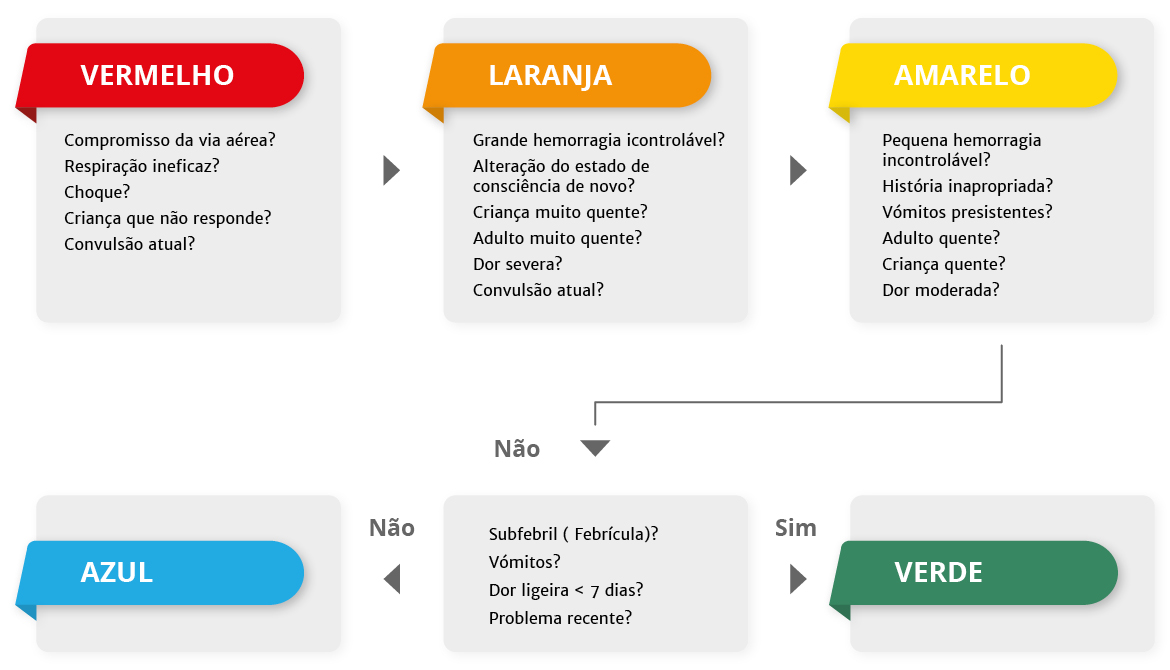
\includegraphics[width=0.9\linewidth]{img/Codigo-Cores-Atendimento-Sistema-Triagem-Manchester.jpg}  % largura percentual 
	\caption{Fluxograma da Triagem de Manchester}
	\label{fig:ccasTriagenManchester}
\end{figure}



\subsection{Testes unitários}


texto para Testes unitários...
 
\colorbox{red}{\Large falta desenvolver mais...}


\subsection{Teste do API: Swagger}


texto para Teste do API: Swagger...
 
\colorbox{red}{\Large falta desenvolver mais...}


\subsection{Teste do API: Postman}


texto para Teste do API: Postman...
 
\colorbox{red}{\Large falta desenvolver mais...}



\subsection{Documentação do API}


texto para Documentação do API...
 
\colorbox{red}{\Large falta desenvolver mais...}


